\documentclass[twoside]{book}

% Packages required by doxygen
\usepackage{calc}
\usepackage{doxygen}
\usepackage{graphicx}
\usepackage[utf8]{inputenc}
\usepackage{makeidx}
\usepackage{multicol}
\usepackage{multirow}
\usepackage{textcomp}
\usepackage[table]{xcolor}

% Font selection
\usepackage[T1]{fontenc}
\usepackage{mathptmx}
\usepackage[scaled=.90]{helvet}
\usepackage{courier}
\usepackage{amssymb}
\usepackage{sectsty}
\renewcommand{\familydefault}{\sfdefault}
\allsectionsfont{%
  \fontseries{bc}\selectfont%
  \color{darkgray}%
}
\renewcommand{\DoxyLabelFont}{%
  \fontseries{bc}\selectfont%
  \color{darkgray}%
}

% Page & text layout
\usepackage{geometry}
\geometry{%
  a4paper,%
  top=2.5cm,%
  bottom=2.5cm,%
  left=2.5cm,%
  right=2.5cm%
}
\tolerance=750
\hfuzz=15pt
\hbadness=750
\setlength{\emergencystretch}{15pt}
\setlength{\parindent}{0cm}
\setlength{\parskip}{0.2cm}
\makeatletter
\renewcommand{\paragraph}{%
  \@startsection{paragraph}{4}{0ex}{-1.0ex}{1.0ex}{%
    \normalfont\normalsize\bfseries\SS@parafont%
  }%
}
\renewcommand{\subparagraph}{%
  \@startsection{subparagraph}{5}{0ex}{-1.0ex}{1.0ex}{%
    \normalfont\normalsize\bfseries\SS@subparafont%
  }%
}
\makeatother

% Headers & footers
\usepackage{fancyhdr}
\pagestyle{fancyplain}
\fancyhead[LE]{\fancyplain{}{\bfseries\thepage}}
\fancyhead[CE]{\fancyplain{}{}}
\fancyhead[RE]{\fancyplain{}{\bfseries\leftmark}}
\fancyhead[LO]{\fancyplain{}{\bfseries\rightmark}}
\fancyhead[CO]{\fancyplain{}{}}
\fancyhead[RO]{\fancyplain{}{\bfseries\thepage}}
\fancyfoot[LE]{\fancyplain{}{}}
\fancyfoot[CE]{\fancyplain{}{}}
\fancyfoot[RE]{\fancyplain{}{\bfseries\scriptsize Generated on Tue Jun 10 2014 22\-:46\-:09 for My Project by Doxygen }}
\fancyfoot[LO]{\fancyplain{}{\bfseries\scriptsize Generated on Tue Jun 10 2014 22\-:46\-:09 for My Project by Doxygen }}
\fancyfoot[CO]{\fancyplain{}{}}
\fancyfoot[RO]{\fancyplain{}{}}
\renewcommand{\footrulewidth}{0.4pt}
\renewcommand{\chaptermark}[1]{%
  \markboth{#1}{}%
}
\renewcommand{\sectionmark}[1]{%
  \markright{\thesection\ #1}%
}

% Indices & bibliography
\usepackage{natbib}
\usepackage[titles]{tocloft}
\setcounter{tocdepth}{3}
\setcounter{secnumdepth}{5}
\makeindex

% Hyperlinks (required, but should be loaded last)
\usepackage{ifpdf}
\ifpdf
  \usepackage[pdftex,pagebackref=true]{hyperref}
\else
  \usepackage[ps2pdf,pagebackref=true]{hyperref}
\fi
\hypersetup{%
  colorlinks=true,%
  linkcolor=blue,%
  citecolor=blue,%
  unicode%
}

% Custom commands
\newcommand{\clearemptydoublepage}{%
  \newpage{\pagestyle{empty}\cleardoublepage}%
}


%===== C O N T E N T S =====

\begin{document}

% Titlepage & ToC
\hypersetup{pageanchor=false}
\pagenumbering{roman}
\begin{titlepage}
\vspace*{7cm}
\begin{center}%
{\Large My Project }\\
\vspace*{1cm}
{\large Generated by Doxygen 1.8.5}\\
\vspace*{0.5cm}
{\small Tue Jun 10 2014 22:46:09}\\
\end{center}
\end{titlepage}
\clearemptydoublepage
\tableofcontents
\clearemptydoublepage
\pagenumbering{arabic}
\hypersetup{pageanchor=true}

%--- Begin generated contents ---
\chapter{R\-E\-A\-D\-M\-E}
\label{md_README}
\hypertarget{md_README}{}
Trabajo de Grado de Oscar Augusto Chamat Caicedo

Este trabajo de grado esta partido en 2 partes cliente y servidor y se mantendra en los repositorios así por simplicidad.

Este cliente es una extension de moodle y utiliza como base el codigo de la aplicación\-: \href{https://github.com/hit-moodle/moodle-local_onlinejudge/blob/master/README.md}{\tt https\-://github.\-com/hit-\/moodle/moodle-\/local\-\_\-onlinejudge/blob/master/\-R\-E\-A\-D\-M\-E.\-md} 
\chapter{Todo List}
\label{todo}
\hypertarget{todo}{}

\begin{DoxyRefList}
\item[\label{todo__todo000001}%
\hypertarget{todo__todo000001}{}%
Member \hyperlink{classlocal__onlinejudge__renderer_ac50ef880eccb084291e5d47ac44d3a47}{local\-\_\-onlinejudge\-\_\-renderer\-:\-:mystatistics} ()]finish it 
\end{DoxyRefList}
\chapter{Namespace Index}
\section{Namespace List}
Here is a list of all documented namespaces with brief descriptions\-:\begin{DoxyCompactList}
\item\contentsline{section}{\hyperlink{namespacelocal__online__uv__judge}{local\-\_\-online\-\_\-uv\-\_\-judge} }{\pageref{namespacelocal__online__uv__judge}}{}
\end{DoxyCompactList}

\chapter{Hierarchical Index}
\section{Class Hierarchy}
This inheritance list is sorted roughly, but not completely, alphabetically\-:\begin{DoxyCompactList}
\item \contentsline{section}{D}{\pageref{classD}}{}
\item \contentsline{section}{Documentation\-Check}{\pageref{classDocumentationCheck}}{}
\item \contentsline{section}{File\-Navigator}{\pageref{classFileNavigator}}{}
\begin{DoxyCompactList}
\item \contentsline{section}{C\-P\-P\-File\-Navigator}{\pageref{classCPPFileNavigator}}{}
\item \contentsline{section}{Scheme\-File\-Navigator}{\pageref{classSchemeFileNavigator}}{}
\end{DoxyCompactList}
\item \contentsline{section}{File\-Navigator\-Factory}{\pageref{classFileNavigatorFactory}}{}
\item \contentsline{section}{Node}{\pageref{classNode}}{}
\item \contentsline{section}{Tree}{\pageref{classTree}}{}
\end{DoxyCompactList}

\chapter{Class Index}
\section{Class List}
Here are the classes, structs, unions and interfaces with brief descriptions\-:\begin{DoxyCompactList}
\item\contentsline{section}{\hyperlink{classjudge__base}{judge\-\_\-base} }{\pageref{classjudge__base}}{}
\item\contentsline{section}{\hyperlink{classlocal__onlinejudge__renderer}{local\-\_\-onlinejudge\-\_\-renderer} }{\pageref{classlocal__onlinejudge__renderer}}{}
\item\contentsline{section}{\hyperlink{classonlinejudge__exception}{onlinejudge\-\_\-exception} }{\pageref{classonlinejudge__exception}}{}
\end{DoxyCompactList}

\chapter{Namespace Documentation}
\hypertarget{namespacelocal__online__uv__judge}{\section{local\-\_\-online\-\_\-uv\-\_\-judge Namespace Reference}
\label{namespacelocal__online__uv__judge}\index{local\-\_\-online\-\_\-uv\-\_\-judge@{local\-\_\-online\-\_\-uv\-\_\-judge}}
}


\subsection{Detailed Description}
\begin{DoxyAuthor}{Author}
Sun Zhigang, Oscar Chamat  \href{http://www.gnu.org/copyleft/gpl.html}{\tt http\-://www.\-gnu.\-org/copyleft/gpl.\-html} G\-N\-U G\-P\-L v3 or later 
\end{DoxyAuthor}

\chapter{Class Documentation}
\hypertarget{classjudge__base}{\section{judge\-\_\-base Class Reference}
\label{classjudge__base}\index{judge\-\_\-base@{judge\-\_\-base}}
}
\subsection*{Public Member Functions}
\begin{DoxyCompactItemize}
\item 
\hypertarget{classjudge__base_a657dfe7c7b40926f36b41d2694dcb3a2}{{\bfseries \-\_\-\-\_\-construct} (\$task)}\label{classjudge__base_a657dfe7c7b40926f36b41d2694dcb3a2}

\item 
\hyperlink{classjudge__base_a5de54be3bb7d6eaf4f99db87ab9074d0}{judge} ()
\end{DoxyCompactItemize}
\subsection*{Static Public Member Functions}
\begin{DoxyCompactItemize}
\item 
static \hyperlink{classjudge__base_a3ec6284e7ab117f88e9ac8590f5a7984}{get\-\_\-languages} ()
\item 
static \hyperlink{classjudge__base_abcb84ebdef8bd20fbd517c37ea09d162}{parse\-\_\-options} (\$options, \&\$task)
\item 
static \hyperlink{classjudge__base_a67f8533487464f6b877981585a8c6bc4}{get\-\_\-compiler\-\_\-info} (\$language)
\item 
static \hyperlink{classjudge__base_a61fce49424ae08c6d3edccf6f8cc768f}{is\-\_\-available} ()
\end{DoxyCompactItemize}
\subsection*{Protected Member Functions}
\begin{DoxyCompactItemize}
\item 
\hyperlink{classjudge__base_abf16f4357be502834cd1415067479581}{convert\-\_\-to\-\_\-utf8} (\$string)
\item 
\hyperlink{classjudge__base_a01360820e47c36821fca6c45e5f259e3}{diff} ()
\item 
\hyperlink{classjudge__base_a72ad9e732c1f6317999bc6ab89f8b5a0}{create\-\_\-temp\-\_\-files} ()
\end{DoxyCompactItemize}
\subsection*{Protected Attributes}
\begin{DoxyCompactItemize}
\item 
\hypertarget{classjudge__base_a077af7aad9f07ad59923330e973023b4}{{\bfseries \$task}}\label{classjudge__base_a077af7aad9f07ad59923330e973023b4}

\item 
\hypertarget{classjudge__base_a35ece71599e0fb37b864cb4854956c68}{{\bfseries \$language}}\label{classjudge__base_a35ece71599e0fb37b864cb4854956c68}

\end{DoxyCompactItemize}


\subsection{Member Function Documentation}
\hypertarget{classjudge__base_abf16f4357be502834cd1415067479581}{\index{judge\-\_\-base@{judge\-\_\-base}!convert\-\_\-to\-\_\-utf8@{convert\-\_\-to\-\_\-utf8}}
\index{convert\-\_\-to\-\_\-utf8@{convert\-\_\-to\-\_\-utf8}!judge_base@{judge\-\_\-base}}
\subsubsection[{convert\-\_\-to\-\_\-utf8}]{\setlength{\rightskip}{0pt plus 5cm}judge\-\_\-base\-::convert\-\_\-to\-\_\-utf8 (
\begin{DoxyParamCaption}
\item[{}]{\$string}
\end{DoxyParamCaption}
)\hspace{0.3cm}{\ttfamily [protected]}}}\label{classjudge__base_abf16f4357be502834cd1415067479581}
If string is not encoded in U\-T\-F-\/8, convert it into utf-\/8 charset \hypertarget{classjudge__base_a72ad9e732c1f6317999bc6ab89f8b5a0}{\index{judge\-\_\-base@{judge\-\_\-base}!create\-\_\-temp\-\_\-files@{create\-\_\-temp\-\_\-files}}
\index{create\-\_\-temp\-\_\-files@{create\-\_\-temp\-\_\-files}!judge_base@{judge\-\_\-base}}
\subsubsection[{create\-\_\-temp\-\_\-files}]{\setlength{\rightskip}{0pt plus 5cm}judge\-\_\-base\-::create\-\_\-temp\-\_\-files (
\begin{DoxyParamCaption}
{}
\end{DoxyParamCaption}
)\hspace{0.3cm}{\ttfamily [protected]}}}\label{classjudge__base_a72ad9e732c1f6317999bc6ab89f8b5a0}
Save files of current task to a temp directory

\begin{DoxyReturn}{Returns}
array of the full path of saved files 
\end{DoxyReturn}
\hypertarget{classjudge__base_a01360820e47c36821fca6c45e5f259e3}{\index{judge\-\_\-base@{judge\-\_\-base}!diff@{diff}}
\index{diff@{diff}!judge_base@{judge\-\_\-base}}
\subsubsection[{diff}]{\setlength{\rightskip}{0pt plus 5cm}judge\-\_\-base\-::diff (
\begin{DoxyParamCaption}
{}
\end{DoxyParamCaption}
)\hspace{0.3cm}{\ttfamily [protected]}}}\label{classjudge__base_a01360820e47c36821fca6c45e5f259e3}
Compare the stdout of program and the output of testcase \hypertarget{classjudge__base_a67f8533487464f6b877981585a8c6bc4}{\index{judge\-\_\-base@{judge\-\_\-base}!get\-\_\-compiler\-\_\-info@{get\-\_\-compiler\-\_\-info}}
\index{get\-\_\-compiler\-\_\-info@{get\-\_\-compiler\-\_\-info}!judge_base@{judge\-\_\-base}}
\subsubsection[{get\-\_\-compiler\-\_\-info}]{\setlength{\rightskip}{0pt plus 5cm}static judge\-\_\-base\-::get\-\_\-compiler\-\_\-info (
\begin{DoxyParamCaption}
\item[{}]{\$language}
\end{DoxyParamCaption}
)\hspace{0.3cm}{\ttfamily [static]}}}\label{classjudge__base_a67f8533487464f6b877981585a8c6bc4}
Return the infomation of the compiler of specified language


\begin{DoxyParams}[1]{Parameters}
string & {\em \$language} & I\-D of the language \\
\hline
\end{DoxyParams}
\begin{DoxyReturn}{Returns}
compiler information or null 
\end{DoxyReturn}
\hypertarget{classjudge__base_a3ec6284e7ab117f88e9ac8590f5a7984}{\index{judge\-\_\-base@{judge\-\_\-base}!get\-\_\-languages@{get\-\_\-languages}}
\index{get\-\_\-languages@{get\-\_\-languages}!judge_base@{judge\-\_\-base}}
\subsubsection[{get\-\_\-languages}]{\setlength{\rightskip}{0pt plus 5cm}static judge\-\_\-base\-::get\-\_\-languages (
\begin{DoxyParamCaption}
{}
\end{DoxyParamCaption}
)\hspace{0.3cm}{\ttfamily [static]}}}\label{classjudge__base_a3ec6284e7ab117f88e9ac8590f5a7984}
Return an array of programming languages supported by this judge

The array key must be the language's I\-D, such as c\-\_\-sandbox, python\-\_\-ideone. The array value must be a human-\/readable name of the language, such as 'C (local)', 'Python (ideone.\-com)' \hypertarget{classjudge__base_a61fce49424ae08c6d3edccf6f8cc768f}{\index{judge\-\_\-base@{judge\-\_\-base}!is\-\_\-available@{is\-\_\-available}}
\index{is\-\_\-available@{is\-\_\-available}!judge_base@{judge\-\_\-base}}
\subsubsection[{is\-\_\-available}]{\setlength{\rightskip}{0pt plus 5cm}static judge\-\_\-base\-::is\-\_\-available (
\begin{DoxyParamCaption}
{}
\end{DoxyParamCaption}
)\hspace{0.3cm}{\ttfamily [static]}}}\label{classjudge__base_a61fce49424ae08c6d3edccf6f8cc768f}
Whether the judge is avaliable

\begin{DoxyReturn}{Returns}
true for yes, false for no 
\end{DoxyReturn}
\hypertarget{classjudge__base_a5de54be3bb7d6eaf4f99db87ab9074d0}{\index{judge\-\_\-base@{judge\-\_\-base}!judge@{judge}}
\index{judge@{judge}!judge_base@{judge\-\_\-base}}
\subsubsection[{judge}]{\setlength{\rightskip}{0pt plus 5cm}judge\-\_\-base\-::judge (
\begin{DoxyParamCaption}
{}
\end{DoxyParamCaption}
)}}\label{classjudge__base_a5de54be3bb7d6eaf4f99db87ab9074d0}
Judge the current task

\begin{DoxyReturn}{Returns}
updated task or false 
\end{DoxyReturn}
\hypertarget{classjudge__base_abcb84ebdef8bd20fbd517c37ea09d162}{\index{judge\-\_\-base@{judge\-\_\-base}!parse\-\_\-options@{parse\-\_\-options}}
\index{parse\-\_\-options@{parse\-\_\-options}!judge_base@{judge\-\_\-base}}
\subsubsection[{parse\-\_\-options}]{\setlength{\rightskip}{0pt plus 5cm}static judge\-\_\-base\-::parse\-\_\-options (
\begin{DoxyParamCaption}
\item[{}]{\$options, }
\item[{\&}]{\$task}
\end{DoxyParamCaption}
)\hspace{0.3cm}{\ttfamily [static]}}}\label{classjudge__base_abcb84ebdef8bd20fbd517c37ea09d162}
Put options into task


\begin{DoxyParams}{Parameters}
{\em object} & options \\
\hline
\end{DoxyParams}
\begin{DoxyReturn}{Returns}
throw exceptions on error 
\end{DoxyReturn}


The documentation for this class was generated from the following file\-:\begin{DoxyCompactItemize}
\item 
judgelib.\-php\end{DoxyCompactItemize}

\hypertarget{classlocal__onlinejudge__renderer}{\section{local\-\_\-onlinejudge\-\_\-renderer Class Reference}
\label{classlocal__onlinejudge__renderer}\index{local\-\_\-onlinejudge\-\_\-renderer@{local\-\_\-onlinejudge\-\_\-renderer}}
}
Inheritance diagram for local\-\_\-onlinejudge\-\_\-renderer\-:\begin{figure}[H]
\begin{center}
\leavevmode
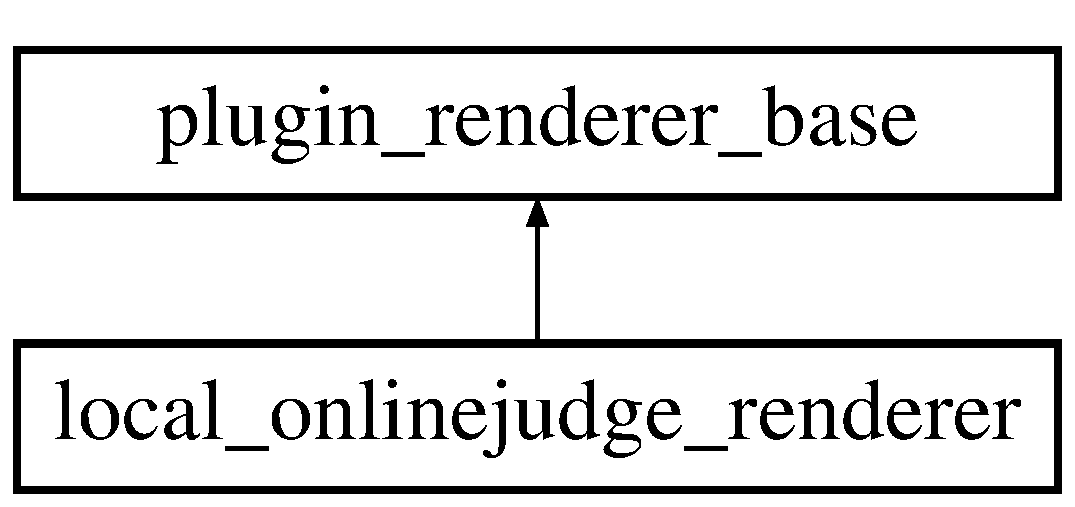
\includegraphics[height=2.000000cm]{classlocal__onlinejudge__renderer}
\end{center}
\end{figure}
\subsection*{Public Member Functions}
\begin{DoxyCompactItemize}
\item 
\hyperlink{classlocal__onlinejudge__renderer_aeecc0ab290a0e44ccfcda4531edd91ca}{judgestatus} ()
\item 
\hyperlink{classlocal__onlinejudge__renderer_ac50ef880eccb084291e5d47ac44d3a47}{mystatistics} ()
\end{DoxyCompactItemize}


\subsection{Detailed Description}
O\-J renderer class 

\subsection{Member Function Documentation}
\hypertarget{classlocal__onlinejudge__renderer_aeecc0ab290a0e44ccfcda4531edd91ca}{\index{local\-\_\-onlinejudge\-\_\-renderer@{local\-\_\-onlinejudge\-\_\-renderer}!judgestatus@{judgestatus}}
\index{judgestatus@{judgestatus}!local_onlinejudge_renderer@{local\-\_\-onlinejudge\-\_\-renderer}}
\subsubsection[{judgestatus}]{\setlength{\rightskip}{0pt plus 5cm}local\-\_\-onlinejudge\-\_\-renderer\-::judgestatus (
\begin{DoxyParamCaption}
{}
\end{DoxyParamCaption}
)}}\label{classlocal__onlinejudge__renderer_aeecc0ab290a0e44ccfcda4531edd91ca}
Renders the online judge status

\begin{DoxyReturn}{Returns}
string 
\end{DoxyReturn}
\hypertarget{classlocal__onlinejudge__renderer_ac50ef880eccb084291e5d47ac44d3a47}{\index{local\-\_\-onlinejudge\-\_\-renderer@{local\-\_\-onlinejudge\-\_\-renderer}!mystatistics@{mystatistics}}
\index{mystatistics@{mystatistics}!local_onlinejudge_renderer@{local\-\_\-onlinejudge\-\_\-renderer}}
\subsubsection[{mystatistics}]{\setlength{\rightskip}{0pt plus 5cm}local\-\_\-onlinejudge\-\_\-renderer\-::mystatistics (
\begin{DoxyParamCaption}
{}
\end{DoxyParamCaption}
)}}\label{classlocal__onlinejudge__renderer_ac50ef880eccb084291e5d47ac44d3a47}
Renders the current user's statistics

\begin{DoxyRefDesc}{Todo}
\item[\hyperlink{todo__todo000001}{Todo}]finish it \end{DoxyRefDesc}
\begin{DoxyReturn}{Returns}
string 
\end{DoxyReturn}


The documentation for this class was generated from the following file\-:\begin{DoxyCompactItemize}
\item 
renderer.\-php\end{DoxyCompactItemize}

\hypertarget{classonlinejudge__exception}{\section{onlinejudge\-\_\-exception Class Reference}
\label{classonlinejudge__exception}\index{onlinejudge\-\_\-exception@{onlinejudge\-\_\-exception}}
}
Inheritance diagram for onlinejudge\-\_\-exception\-:\begin{figure}[H]
\begin{center}
\leavevmode
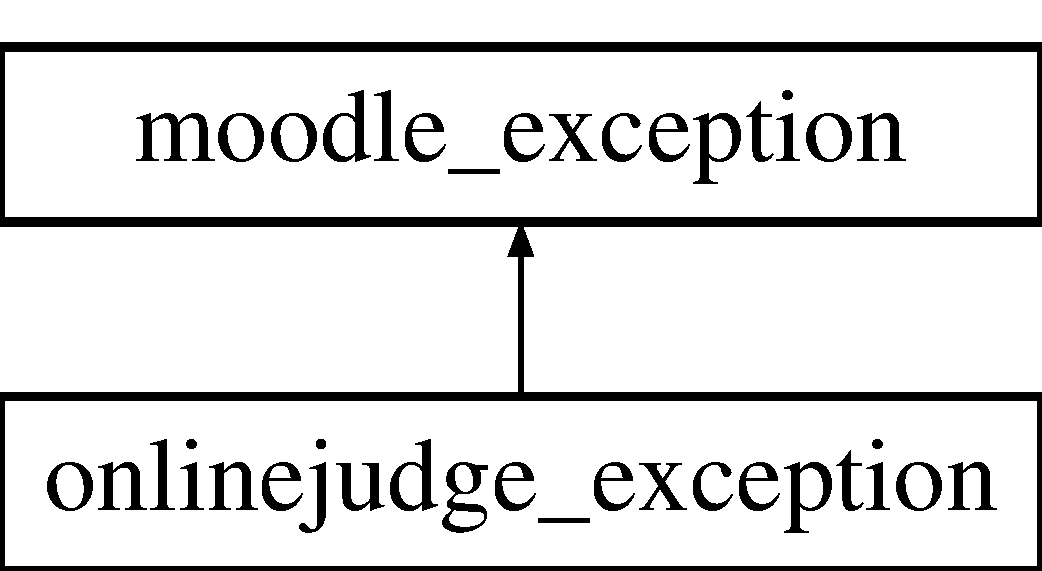
\includegraphics[height=2.000000cm]{classonlinejudge__exception}
\end{center}
\end{figure}
\subsection*{Public Member Functions}
\begin{DoxyCompactItemize}
\item 
\hypertarget{classonlinejudge__exception_ae174ebe037099e6d9a2fa16633809e5e}{{\bfseries \-\_\-\-\_\-construct} (\$errorcode, \$a=N\-U\-L\-L, \$debuginfo=N\-U\-L\-L)}\label{classonlinejudge__exception_ae174ebe037099e6d9a2fa16633809e5e}

\end{DoxyCompactItemize}


The documentation for this class was generated from the following file\-:\begin{DoxyCompactItemize}
\item 
exceptions.\-php\end{DoxyCompactItemize}

%--- End generated contents ---

% Index
\newpage
\phantomsection
\addcontentsline{toc}{part}{Index}
\printindex

\end{document}
